% Created 2025-06-30 Mon 15:33
% Intended LaTeX compiler: pdflatex
\documentclass[bigger,aspectratio=169]{beamer}
  \usepackage{caption, subcaption, csquotes, amssymb, xcolor, svg}
\usepackage[english]{babel}
\titlegraphic{\includesvg[height=1cm]{./figs/IE_Unicamp}\hspace*{1.25cm}\includesvg[height=1cm]{./figs/SSSA}\hspace*{1.25cm} \includesvg[height=1cm]{./figs/YSI}}
\AtBeginSection[]{
\begin{frame}{Outline}
\tableofcontents[currentsection]
\end{frame}
}
\usepackage[utf8]{inputenc}
\usepackage[T1]{fontenc}
\usepackage{amsmath}
\usepackage{amsfonts}
\usepackage{amssymb}
\usepackage{multicol}
\usepackage{graphicx}
\usepackage{textpos}
\usepackage{caption}
\usepackage{subfig}
\usepackage{svg}
\usepackage{pgfpages}
\usepackage{epstopdf}
\epstopdfsetup{update} % only regenerate if changed
\DeclareGraphicsRule{.eps}{pdf}{.pdf}{`epstopdf #1}
\usepackage{tikz}
\usetikzlibrary{arrows.meta, positioning, shapes}
\usepackage{fontawesome5}
\usetheme{metropolis}
\usecolortheme{beaver}
\author{Gabriel Petrini}
\date{July, 2025}
\title{ABM Macro Lab: Agent-based Modelling Tools}
\subtitle{Session 03}
\hypersetup{
 pdfauthor={Gabriel Petrini},
 pdftitle={ABM Macro Lab: Agent-based Modelling Tools},
 pdfkeywords={},
 pdfsubject={},
 pdfcreator={Emacs 29.3 (Org mode 9.7.31)}, 
 pdflang={English}}

% Setup for code blocks [1/2]

\usepackage{fvextra}

\fvset{%
  commandchars=\\\{\},
  highlightcolor=white!95!black!80!blue,
  breaklines=true,
  breaksymbol=\color{white!60!black}\tiny\ensuremath{\hookrightarrow}}

% Make line numbers smaller and grey.
\renewcommand\theFancyVerbLine{\footnotesize\color{black!40!white}\arabic{FancyVerbLine}}

\usepackage{xcolor}

% In case engrave-faces-latex-gen-preamble has not been run.
\providecolor{EfD}{HTML}{f7f7f7}
\providecolor{EFD}{HTML}{28292e}

% Define a Code environment to prettily wrap the fontified code.
\usepackage[breakable,xparse]{tcolorbox}
\DeclareTColorBox[]{Code}{o}%
{colback=EfD!98!EFD, colframe=EfD!95!EFD,
  fontupper=\footnotesize\setlength{\fboxsep}{0pt},
  colupper=EFD,
  IfNoValueTF={#1}%
  {boxsep=2pt, arc=2.5pt, outer arc=2.5pt,
    boxrule=0.5pt, left=2pt}%
  {boxsep=2.5pt, arc=0pt, outer arc=0pt,
    boxrule=0pt, leftrule=1.5pt, left=0.5pt},
  right=2pt, top=1pt, bottom=0.5pt,
  breakable}

% Support listings with captions
\usepackage{float}
\floatstyle{plain}
\newfloat{listing}{htbp}{lst}
\newcommand{\listingsname}{Listing}
\floatname{listing}{\listingsname}
\newcommand{\listoflistingsname}{List of Listings}
\providecommand{\listoflistings}{\listof{listing}{\listoflistingsname}}


% Setup for code blocks [2/2]: syntax highlighting colors

\newcommand\efstrut{\vrule height 2.1ex depth 0.8ex width 0pt}
\definecolor{EFD}{HTML}{383a42}
\definecolor{EfD}{HTML}{fafafa}
\newcommand{\EFD}[1]{\textcolor{EFD}{#1}} % default
\newcommand{\EFvp}[1]{#1} % variable-pitch
\definecolor{EFh}{HTML}{9ca0a4}
\newcommand{\EFh}[1]{\textcolor{EFh}{#1}} % shadow
\definecolor{EFsc}{HTML}{50a14f}
\newcommand{\EFsc}[1]{\textcolor{EFsc}{#1}} % success
\definecolor{EFw}{HTML}{986801}
\newcommand{\EFw}[1]{\textcolor{EFw}{#1}} % warning
\definecolor{EFe}{HTML}{e45649}
\newcommand{\EFe}[1]{\textcolor{EFe}{#1}} % error
\definecolor{Efl}{HTML}{c6c7c7}
\newcommand{\EFl}[1]{\colorbox{Efl}{\efstrut{}\textbf{#1}}} % link
\definecolor{EFlv}{HTML}{8b008b}
\definecolor{Eflv}{HTML}{c6c7c7}
\newcommand{\EFlv}[1]{\colorbox{Eflv}{\efstrut{}\textcolor{EFlv}{\textbf{#1}}}} % link-visited
\definecolor{EFhi}{HTML}{f0f0f0}
\definecolor{Efhi}{HTML}{4078f2}
\newcommand{\EFhi}[1]{\colorbox{Efhi}{\efstrut{}\textcolor{EFhi}{#1}}} % highlight
\definecolor{EFc}{HTML}{9ca0a4}
\newcommand{\EFc}[1]{\textcolor{EFc}{#1}} % font-lock-comment-face
\definecolor{EFcd}{HTML}{9ca0a4}
\newcommand{\EFcd}[1]{\textcolor{EFcd}{#1}} % font-lock-comment-delimiter-face
\definecolor{EFs}{HTML}{50a14f}
\newcommand{\EFs}[1]{\textcolor{EFs}{#1}} % font-lock-string-face
\definecolor{EFd}{HTML}{84888b}
\newcommand{\EFd}[1]{\textcolor{EFd}{\textit{#1}}} % font-lock-doc-face
\definecolor{EFm}{HTML}{b751b6}
\newcommand{\EFm}[1]{\textcolor{EFm}{#1}} % font-lock-doc-markup-face
\definecolor{EFk}{HTML}{e45649}
\newcommand{\EFk}[1]{\textcolor{EFk}{#1}} % font-lock-keyword-face
\definecolor{EFb}{HTML}{a626a4}
\newcommand{\EFb}[1]{\textcolor{EFb}{#1}} % font-lock-builtin-face
\definecolor{EFf}{HTML}{a626a4}
\newcommand{\EFf}[1]{\textcolor{EFf}{#1}} % font-lock-function-name-face
\definecolor{EFv}{HTML}{6a1868}
\newcommand{\EFv}[1]{\textcolor{EFv}{#1}} % font-lock-variable-name-face
\definecolor{EFt}{HTML}{986801}
\newcommand{\EFt}[1]{\textcolor{EFt}{#1}} % font-lock-type-face
\definecolor{EFo}{HTML}{b751b6}
\newcommand{\EFo}[1]{\textcolor{EFo}{#1}} % font-lock-constant-face
\definecolor{EFwr}{HTML}{986801}
\newcommand{\EFwr}[1]{\textcolor{EFwr}{#1}} % font-lock-warning-face
\definecolor{EFnc}{HTML}{4078f2}
\newcommand{\EFnc}[1]{\textcolor{EFnc}{\textbf{#1}}} % font-lock-negation-char-face
\definecolor{EFpp}{HTML}{4078f2}
\newcommand{\EFpp}[1]{\textcolor{EFpp}{\textbf{#1}}} % font-lock-preprocessor-face
\definecolor{EFrc}{HTML}{4078f2}
\newcommand{\EFrc}[1]{\textcolor{EFrc}{\textbf{#1}}} % font-lock-regexp-grouping-construct
\definecolor{EFrb}{HTML}{4078f2}
\newcommand{\EFrb}[1]{\textcolor{EFrb}{\textbf{#1}}} % font-lock-regexp-grouping-backslash
\definecolor{Efob}{HTML}{e7e7e7}
\newcommand{\EFob}[1]{\colorbox{Efob}{\efstrut{}#1}} % org-block
\definecolor{Efobb}{HTML}{e7e7e7}
\newcommand{\EFobb}[1]{\colorbox{Efobb}{\efstrut{}\textit{#1}}} % org-block-begin-line
\definecolor{Efobe}{HTML}{e7e7e7}
\newcommand{\EFobe}[1]{\colorbox{Efobe}{\efstrut{}\textit{#1}}} % org-block-end-line
\definecolor{EFOa}{HTML}{e45649}
\newcommand{\EFOa}[1]{\textcolor{EFOa}{\textbf{#1}}} % outline-1
\definecolor{EFOb}{HTML}{da8548}
\newcommand{\EFOb}[1]{\textcolor{EFOb}{\textbf{#1}}} % outline-2
\definecolor{EFOc}{HTML}{b751b6}
\newcommand{\EFOc}[1]{\textcolor{EFOc}{\textbf{#1}}} % outline-3
\definecolor{EFOd}{HTML}{6f99f5}
\newcommand{\EFOd}[1]{\textcolor{EFOd}{\textbf{#1}}} % outline-4
\definecolor{EFOe}{HTML}{bc5cba}
\newcommand{\EFOe}[1]{\textcolor{EFOe}{\textbf{#1}}} % outline-5
\definecolor{EFOf}{HTML}{9fbbf8}
\newcommand{\EFOf}[1]{\textcolor{EFOf}{\textbf{#1}}} % outline-6
\definecolor{EFOg}{HTML}{d292d1}
\newcommand{\EFOg}[1]{\textcolor{EFOg}{\textbf{#1}}} % outline-7
\definecolor{EFOh}{HTML}{d8e4fc}
\newcommand{\EFOh}[1]{\textcolor{EFOh}{\textbf{#1}}} % outline-8
\newcommand{\EFhn}[1]{#1} % highlight-numbers-number
\newcommand{\EFhq}[1]{#1} % highlight-quoted-quote
\newcommand{\EFhs}[1]{#1} % highlight-quoted-symbol
\newcommand{\EFrda}[1]{#1} % rainbow-delimiters-depth-1-face
\newcommand{\EFrdb}[1]{#1} % rainbow-delimiters-depth-2-face
\newcommand{\EFrdc}[1]{#1} % rainbow-delimiters-depth-3-face
\newcommand{\EFrdd}[1]{#1} % rainbow-delimiters-depth-4-face
\newcommand{\EFrde}[1]{#1} % rainbow-delimiters-depth-5-face
\newcommand{\EFrdf}[1]{#1} % rainbow-delimiters-depth-6-face
\newcommand{\EFrdg}[1]{#1} % rainbow-delimiters-depth-7-face
\newcommand{\EFrdh}[1]{#1} % rainbow-delimiters-depth-8-face
\newcommand{\EFrdi}[1]{#1} % rainbow-delimiters-depth-9-face
\definecolor{EFany}{HTML}{986801}
\definecolor{Efany}{HTML}{986801}
\newcommand{\EFany}[1]{\colorbox{Efany}{\efstrut{}\textcolor{EFany}{#1}}} % ansi-color-yellow
\definecolor{EFanr}{HTML}{e45649}
\definecolor{Efanr}{HTML}{e45649}
\newcommand{\EFanr}[1]{\colorbox{Efanr}{\efstrut{}\textcolor{EFanr}{#1}}} % ansi-color-red
\definecolor{EFanb}{HTML}{fafafa}
\newcommand{\EFanb}[1]{\textcolor{EFanb}{#1}} % ansi-color-black
\definecolor{EFang}{HTML}{50a14f}
\definecolor{Efang}{HTML}{50a14f}
\newcommand{\EFang}[1]{\colorbox{Efang}{\efstrut{}\textcolor{EFang}{#1}}} % ansi-color-green
\definecolor{EFanB}{HTML}{4078f2}
\definecolor{EfanB}{HTML}{4078f2}
\newcommand{\EFanB}[1]{\colorbox{EfanB}{\efstrut{}\textcolor{EFanB}{#1}}} % ansi-color-blue
\definecolor{EFanc}{HTML}{0184bc}
\definecolor{Efanc}{HTML}{0184bc}
\newcommand{\EFanc}[1]{\colorbox{Efanc}{\efstrut{}\textcolor{EFanc}{#1}}} % ansi-color-cyan
\definecolor{Efanw}{HTML}{383a42}
\newcommand{\EFanw}[1]{\colorbox{Efanw}{\efstrut{}#1}} % ansi-color-white
\definecolor{EFanm}{HTML}{a626a4}
\definecolor{Efanm}{HTML}{a626a4}
\newcommand{\EFanm}[1]{\colorbox{Efanm}{\efstrut{}\textcolor{EFanm}{#1}}} % ansi-color-magenta
\definecolor{EFANy}{HTML}{a77e27}
\definecolor{EfANy}{HTML}{a77e27}
\newcommand{\EFANy}[1]{\colorbox{EfANy}{\efstrut{}\textcolor{EFANy}{#1}}} % ansi-color-bright-yellow
\definecolor{EFANr}{HTML}{e86f64}
\definecolor{EfANr}{HTML}{e86f64}
\newcommand{\EFANr}[1]{\colorbox{EfANr}{\efstrut{}\textcolor{EFANr}{#1}}} % ansi-color-bright-red
\definecolor{EFANb}{HTML}{9ca0a4}
\definecolor{EfANb}{HTML}{9ca0a4}
\newcommand{\EFANb}[1]{\colorbox{EfANb}{\efstrut{}\textcolor{EFANb}{#1}}} % ansi-color-bright-black
\definecolor{EFANg}{HTML}{6aaf69}
\definecolor{EfANg}{HTML}{6aaf69}
\newcommand{\EFANg}[1]{\colorbox{EfANg}{\efstrut{}\textcolor{EFANg}{#1}}} % ansi-color-bright-green
\definecolor{EFANB}{HTML}{5c8cf3}
\definecolor{EfANB}{HTML}{5c8cf3}
\newcommand{\EFANB}[1]{\colorbox{EfANB}{\efstrut{}\textcolor{EFANB}{#1}}} % ansi-color-bright-blue
\definecolor{EFANc}{HTML}{2796c6}
\definecolor{EfANc}{HTML}{2796c6}
\newcommand{\EFANc}[1]{\colorbox{EfANc}{\efstrut{}\textcolor{EFANc}{#1}}} % ansi-color-bright-cyan
\definecolor{EFANw}{HTML}{1b2229}
\definecolor{EfANw}{HTML}{1b2229}
\newcommand{\EFANw}[1]{\colorbox{EfANw}{\efstrut{}\textcolor{EFANw}{#1}}} % ansi-color-bright-white
\definecolor{EFANm}{HTML}{b346b1}
\definecolor{EfANm}{HTML}{b346b1}
\newcommand{\EFANm}[1]{\colorbox{EfANm}{\efstrut{}\textcolor{EFANm}{#1}}} % ansi-color-bright-magenta
\usepackage[style=authoryear]{biblatex}
\addbibresource{~/Org/zotero_refs.bib}
\begin{document}

\maketitle
\begin{frame}{Outline}
\tableofcontents
\end{frame}

\section{Introduction}
\label{sec:org6b671ff}


\begin{frame}[label={sec:org228244f}]{Where are we and where are we going?}
\begin{description}
\item[{Session I}] Basics of LSD and small models implementation
\item[{Session II}] Presentation of the Industry model and implementation
\item[{Session III (Today)}] Q\&A, bug fixes, and analysis of results and Monte Carlo Experiment
\end{description}
\end{frame}
\begin{frame}[label={sec:orga5e5252},fragile]{Lost? I}
 In case you are lost, here are some few-liner to catch up (code may differ)?

\begin{Code}
\begin{Verbatim}
\color{EFD}\EFo{EQUATION}( \EFs{"a"} )
\EFcd{//} \EFc{Firm knowledge/productivity}
\EFo{RESULT}( VL( \EFs{"a"}, 1 ) * ( 1 + V( \EFs{"eta"} ) * beta( V( \EFs{"beta1"} ), V( \EFs{"beta2"} ) ) ) )

\EFo{EQUATION}( \EFs{"s"} )
\EFcd{//} \EFc{Firm size/market share}
\EFo{RESULT}( VL( \EFs{"s"}, 1 ) * ( 1 + V( \EFs{"A"} ) * ( V( \EFs{"a"} ) - V( \EFs{"aAvg"} ) ) / V( \EFs{"aAvg"} ) ) )

\EFo{EQUATION}( \EFs{"HHI"} )
\EFcd{//} \EFc{Herfindahl-Hirschman concentration index}
\EFo{RESULT}( \EFo{WHTAVE}( \EFs{"s"}, \EFs{"s"} ) )

\end{Verbatim}
\end{Code}
\end{frame}
\begin{frame}[label={sec:orgfec052f},fragile]{Lost? II}
 \begin{Code}
\begin{Verbatim}
\color{EFD}\EFo{EQUATION}( \EFs{"exit\_decision"} )
\EFk{if} ( V( \EFs{"s"} ) < V( \EFs{"sMin"} ) ) \{
    \EFo{WRITE}( \EFs{"a"}, V( \EFs{"aAvg"} ) * ( 1 + V( \EFs{"eta"} ) * beta( V( \EFs{"beta1"} ), V( \EFs{"beta2"} ) ) ) );
    \EFo{WRITE}( \EFs{"s"}, 1 / \EFo{COUNT}( \EFs{"Firm"} ) );
\}
\EFo{RESULT}( 0 )

\EFo{EQUATION}( \EFs{"aAvg"} )
\EFcd{//} \EFc{Mean knowledge/productivity}
v[0] = 0;        \EFcd{//} \EFc{accumulator}
\EFo{CYCLE}( cur, \EFs{"Firm"} )
    v[0] += \EFo{VLS}( cur, \EFs{"s"}, 1 ) * VS( cur, \EFs{"a"} );
\EFo{RESULT}( v[0] )
\end{Verbatim}
\end{Code}
\end{frame}
\begin{frame}[label={sec:orgfd90adc},fragile]{Lost? III}
 \begin{Code}
\begin{Verbatim}
\color{EFD}\EFo{EQUATION}( \EFs{"exit\_entry"} )
\EFcd{//} \EFc{Trigger market-wise exit-entry dynamics and re-scale shares}
V( \EFs{"HHI"} ); \EFcd{//} \EFc{first, compute HH index before exits}
\EFo{CYCLE}( cur, \EFs{"Firm"} ) \EFcd{//} \EFc{second, ensure firms have decided on exit}
    VS( cur, \EFs{"exit\_decision"} );
v[0] = 1 / \EFo{SUM}( \EFs{"s"} );\EFcd{//} \EFc{factor to scale back to sum = 1}
\EFo{CYCLE}( cur, \EFs{"Firm"} ) \EFcd{//} \EFc{third, rescale market shares after exits}
    \EFo{WRITES}( cur, \EFs{"s"}, v[0] * VS( cur, \EFs{"s"} ) );
\EFo{RESULT}(0)
\end{Verbatim}
\end{Code}
\end{frame}
\section{Activities}
\label{sec:org87175c1}


\begin{frame}[label={sec:org1ca0ea0},fragile]{Activity I}
 \begin{enumerate}
\item Show that average productivity (\texttt{aAvg}) is always between a maximum and minimum productivities
\item Check that the total market share of firms is constant and equal to 1
\item Increase (1) the number of firms to 150, (2) the exit threshold \texttt{sMin} to 0.001, and the number of simulation steps.
\item Run and analyze the results. What are the main differences?
\item Using this new configuration, produce a \alert{histogram} of the firm log-size distribution at \(t = 200\)
\end{enumerate}
\end{frame}
\begin{frame}[label={sec:orgb88e23b}]{Histogram of firm log-size distribution (\(t = 200\))}
\begin{center}
\includesvg[width=.9\linewidth]{./figs/150_firms_log_size_histogram}
\end{center}
\end{frame}
\begin{frame}[label={sec:org9ef311b}]{A simple Monte Carlo experiment I}
\begin{enumerate}
\item Close Analysis of Results window
\item Re-open the baseline configuration
\item Set the simulation runs to \alert{20} (\alert{Run > Simulation})
\item Save as a new configuration
\item Run the new configuration (\alert{Run > Run})
\item Choose \alert{Data > Analysis of MC Experiment}, accept using last results, and mark to create \alert{Average} and \alert{Maximum and minimum} series, and to include confidence intervals
\item Analyze the Monte Carlo experiment results
\end{enumerate}
\end{frame}
\begin{frame}[label={sec:orgcfd79ed}]{A simple Monte Carlo experiment II}
\begin{center}
\includesvg[width=.9\linewidth]{./figs/HHI_MC}
\end{center}
\end{frame}
\begin{frame}[label={sec:orga5ad440}]{Activity II}
\begin{enumerate}
\item Show the max-min intervals for the average log-productivity (\alert{aAvg}) and the \alert{HHI} in the MC experiment
\item Why the MC confidence width is not comparable for the two variables?
\item Show the distribution of the productivity (\alert{a}) considering all MC runs (tip: select \alert{Keep original series in Monte Carlo options})
\item The Monte Carlo analysis uncovers a potential problem with this simplified version of the model, try to identify it, and to reason if it can invalidate the results obtained
\end{enumerate}
\end{frame}
\section{Simple parameter sensitivity check}
\label{sec:org8c384c2}

\begin{frame}[label={sec:orga7cdb3f}]{Introduction}
In this part of the lecture, we will playaround with \(A\) and \(\eta\) parameters and check their impacts on the model output.
Here, we will leverage the benefits of an OOP design associated with an isolated configuration setting.

In the same way we made copies of a specific firm, we can also make a copy of the whole structure of the model.
By doing this, we can make different experiments on each copy and analyze it on LSD.
\begin{block}{Good news!}
LSD has some ways to automatize this task for us.
\end{block}
\end{frame}
\begin{frame}[label={sec:org8b6b745},fragile]{Setting the DoE I}
 \begin{enumerate}
\item Load \texttt{Sim1.lsd} and save it as \texttt{Sim1\_DoE.lsd}
\item Right click on \texttt{A} and select \alert{Sensitivity}
\item On the new window, specify the parameter range as follows:
\end{enumerate}

\begin{verbatim}
=MIN:MAX@NUM%L
\end{verbatim}

\begin{description}
\item[{MIN}] Minimal value
\item[{MAX}] Maximum value
\item[{NUM}] Number of samples
\item[{\%L}] Indicates to vary linearly
\end{description}

Next, repeat the same for \texttt{eta}
\end{frame}
\begin{frame}[label={sec:org6b03f2d},fragile]{Example of the parametric space}
 \begin{center}
\begin{tabular}{ccccc}
\hline
 & Desc & Baseline & Min & Max\\
\hline
\(\eta\) & Innovation opportunity support & 0.3 & 0.1 & 0.7\\
\(A\) & replicator dynamics intensity & 1 & 0.2 & 5\\
\hline
\end{tabular}
\end{center}
\begin{description}
\item[{eta}] \texttt{=0.1:0.7@3\%L}
\item[{A}] \texttt{=0.2:5@3\%L}
\end{description}
\end{frame}
\begin{frame}[label={sec:org109b9a1},fragile]{Setting the DoE II}
 \begin{enumerate}
\item After, save the sensitivity analysis file (\alert{File>Save sensitivity})
\item Mark \texttt{A} and \texttt{eta} to be saved
\item Set the DoE (\alert{Data > Sensitivity Analysis > Full (Online)})
\item Run the simulations (Run > Run) to produce the results files (accept the defaults)
\item Choose \alert{Data > Analysis of results} and inspects the results
\item Whenever picking a variable to plot, right click on it and choose to select all
\end{enumerate}
\end{frame}
\begin{frame}[label={sec:org847fc11},fragile]{Activity III}
 Set your own parametric ranges (choose an small number for \texttt{NUM}).

\begin{itemize}
\item How can we evaluate the importance of a parameter?
\item How each parameter affects the model's results?
\item What is the economic intuition of this?
\item How can we efficiently repeat this for all other parameters and initial conditions?
\end{itemize}
\end{frame}
\begin{frame}[label={sec:org0ca373e}]{Visualizing this experiment}
\begin{center}
\includesvg[height=.85\textheight]{./figs/Full_DoE.svg}
\end{center}
\end{frame}
\section{Primer on sensitivity analysis (Bonus)}
\label{sec:org3ee2441}

\begin{frame}[label={sec:org0e644fe}]{Model sensitivity to parameters}
How do parameters and initial conditions \alert{jointly} affect variables?

\begin{itemize}
\item The most common approach is to perform a one-variable at a time change
\begin{itemize}
\item In this small-scale model, we can play with different parameters and check
\end{itemize}
\item However, even with this small parametric space, the number of combinations can get quickly large
\item We will briefly check some Design of Experiments Techniques that helps with this situations
\end{itemize}
\end{frame}
\begin{frame}[label={sec:org4ce0c40}]{Sensitivity analysis}
Sensitivity analysis requires many steps:

\begin{enumerate}
\item Screening: Filter down unimportant factors (elementary effects)
\item Select a \alert{Design of Experiments} (DoE) strategy
\item Evaluate multiple runs per configuration
\item If required, fit a \alert{meta-model}
\item Compute the sensitivity analysis \alert{statistics}
\item Explore the \alert{response surfaces}
\end{enumerate}

\alert{Good news:} LSD (+R) can handle this through a NNF approach
\begin{block}{Note on screening}
As the model is small, we will skip screening and jump directly to metamodels
\end{block}
\end{frame}
\begin{frame}[label={sec:orgc17b02e}]{Parametric space}
\begin{center}
\begin{tabular}{ccccc}
\hline
 & Desc & Baseline & Min & Max\\
\hline
\(\eta\) & Innovation opportunity support & 0.3 & 0.0 & 0.7\\
\(\beta_{1}, \beta_{2}\) & beta distribution parameters & 1.0; 5.0 & 1; 3 & 3;10\\
\(A\) & replicator dynamics intensity & 1 & 0.2 & 5\\
\(s_{min}\) & minimum market share to not exit & 0.01 & 0.0001 & 0.01\\
\(NF\) & number of firms & 10 & 10 & 350\\
\hline
\end{tabular}
\end{center}
\begin{block}{Monte Carlo vs Near Orthogonal Latin Hypercube}
\begin{itemize}
\item All combinations possible (MC): 64 (x 5)
\item NOLH: 43 (x 5)
\end{itemize}
\end{block}
\end{frame}
\begin{frame}[label={sec:org45c4f87}]{Exploring the industry model}
Load \href{Industry\_SummerSchool/R/data/Sim-Sobol.lsd}{R/data/Sim-Sobol.lsd} file in LSD
\begin{enumerate}
\item This is a copy of \href{Industry\_SummerSchool/Sim1.lsd}{Sim1.lsd} with 5 simulation runs
\end{enumerate}
\begin{enumerate}
\item Load sensitivity analysis configuration (\alert{File > Load sensitivity\ldots{}}) and choose \href{Industry\_SummerSchool/R/Sim-Sobol.sa}{R/Sim-Sobol.sa}
\item Set the DoE (\alert{Data > Sensitivity Analysis > NOHL sampling})
\begin{enumerate}
\item Select \alert{Extended number of samples}, hit \alert{OK} and accepts the default
\end{enumerate}
\item Run a \alert{parallel batch} (Run > Parallel Batch) to produce the results files (accept the defaults)
\item Let's jump into R(studio) and create a project under the \alert{R} folder
\item Select the \alert{sobol-SA.R} and hit source
\end{enumerate}
\begin{block}{Before checking the results}
Which parameters do you expect to most influence \alert{HHI}? What about \alert{aAvg}?
\end{block}
\end{frame}
\begin{frame}[label={sec:orgeaf3153}]{Sobol decomposition indexes (HHI)}
\begin{center}
\includegraphics[height=.875\textheight,page=4]{./Industry_SummerSchool/R/data/Sim-Sobol_kriging_HHI.pdf}
\end{center}
\end{frame}
\begin{frame}[label={sec:org2bbaf12}]{Meta-model response I}
\begin{center}
\includegraphics[height=.85\textheight,page=5]{./Industry_SummerSchool/R/data/Sim-Sobol_kriging_HHI.pdf}
\end{center}
\end{frame}
\begin{frame}[label={sec:org877370b}]{Meta-model response II}
\begin{center}
\includegraphics[height=.85\textheight,page=6]{./Industry_SummerSchool/R/data/Sim-Sobol_kriging_HHI.pdf}
\end{center}
\end{frame}
\begin{frame}[label={sec:org26a12ee}]{Meta-model response III}
\begin{center}
\includegraphics[height=.85\textheight,page=7]{./Industry_SummerSchool/R/data/Sim-Sobol_kriging_HHI.pdf}
\end{center}
\end{frame}
\begin{frame}[label={sec:org9fcbd00},fragile]{Bonus Activity}
 \begin{itemize}
\item In the Rscript, uncomment \Verb[commandchars=\\\{\},highlightcolor=white!95!black!80!blue,breaklines=true,breaksymbol=\color{white!60!black}\tiny\ensuremath{\hookrightarrow}]{\color{EFD}varName \textcolor[HTML]{008b8b}{<-} \EFs{"aAvg"}} and source the file again
\item Open the resulting PDF file
\item Analyze the results and contrast with your expectations
\item What are the economic intuition associated with these parameters?
\end{itemize}
\end{frame}
\begin{frame}[label={sec:orgef50c8e}]{Phew!}

Our papers are available at:

\faNewspaper\ \texttt{http://www.lem.sssup.it/wplem.html}\\

You can reach me at:

\faEnvelope\ \texttt{gpetrinidasilveira@gmail.com} \\
\faGithub\ \texttt{github.com/gpetrini} \\
\faOrcid & \texttt{https://orcid.org/0000-0002-3523-9826} \\

\\\Huge{Thank you!}
\end{frame}
\end{document}
